% CU-MOBO main conceptual figure (hero).
% Compile:  pdflatex -interaction=nonstopmode main_figure.tex
% PNG:      pdftoppm -png -r 300 main_figure.pdf main_figure
\documentclass[border=8pt]{standalone}
\usepackage{tikz}
\usepackage{amsmath}
\usetikzlibrary{positioning,arrows.meta,calc,backgrounds,fit,shapes.geometric}

\definecolor{cTrue}{RGB}{31,119,180}    % true activity
\definecolor{cMu}{RGB}{214,39,40}       % oracle mu
\definecolor{cBand}{RGB}{255,165,145}   % sigma band
\definecolor{cGood}{RGB}{44,160,44}     % CU-MOBO pick
\definecolor{cTrap}{RGB}{200,30,30}     % naive pick / trap
\definecolor{cBox}{RGB}{60,60,90}
\definecolor{cM1}{RGB}{31,119,180}
\definecolor{cM2}{RGB}{44,160,44}
\definecolor{cM3}{RGB}{148,103,189}

\begin{document}
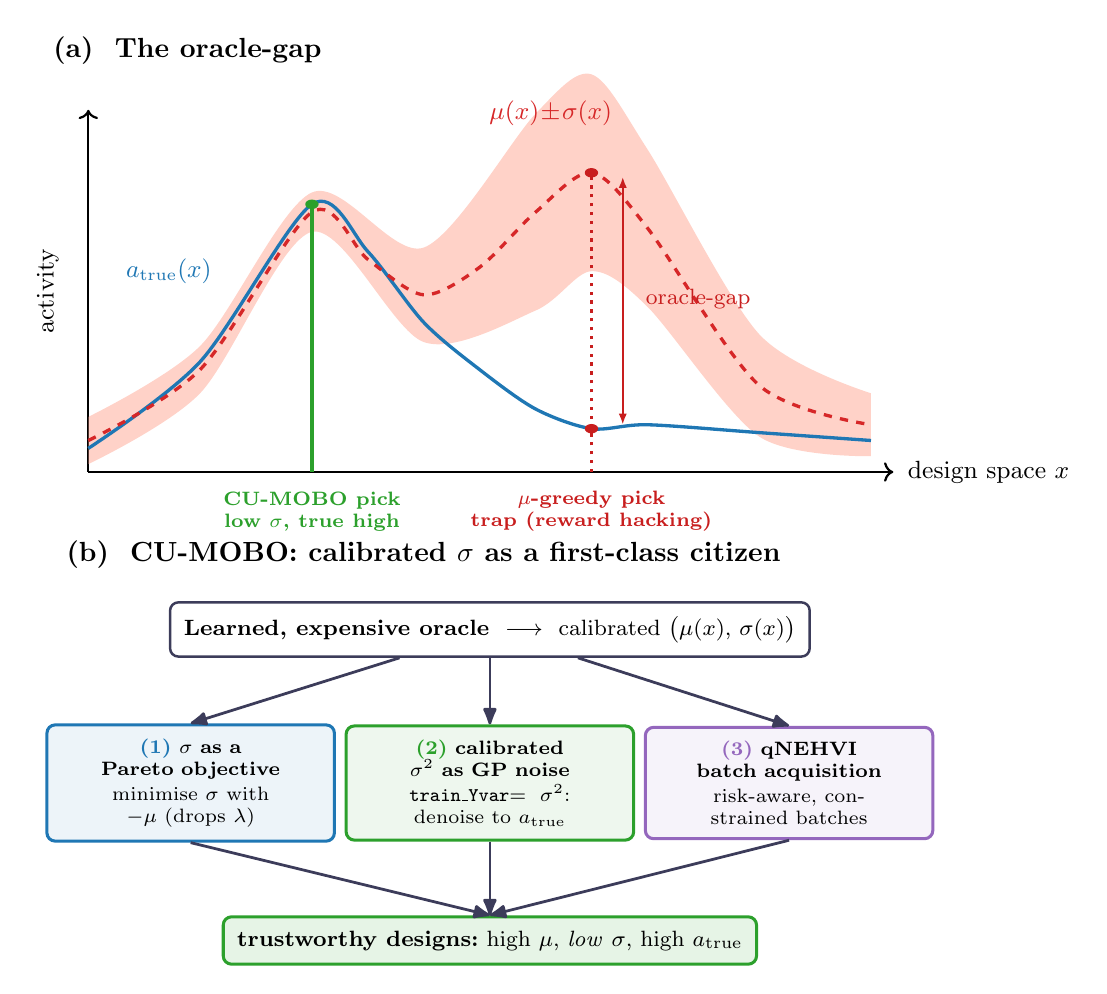
\begin{tikzpicture}[font=\small]

% =========================================================
% Panel (a): the oracle-gap  (top)
% =========================================================
\begin{scope}[yshift=6.3cm,xscale=1.42]
  \def\W{7.2} \def\H{4.6}
  \draw[->,thick] (0,0) -- (\W,0) node[right] {\,design space $x$};
  \draw[->,thick] (0,0) -- (0,\H);
  \node[rotate=90,anchor=south] at (-0.18,\H/2) {activity};

  % sigma band around oracle mu (mu+sigma upper, mu-sigma lower reversed)
  \fill[cBand,opacity=0.5]
    plot[smooth] coordinates {(0.0,0.7)(1.0,1.6)(2.0,3.55)(3.0,2.85)(4.0,4.55)(4.5,5.05)(5.0,4.1)(6.0,1.75)(7.0,1.0)}
    -- plot[smooth] coordinates {(7.0,0.2)(6.0,0.45)(5.0,2.1)(4.5,2.55)(4.0,2.05)(3.0,1.65)(2.0,3.05)(1.0,1.0)(0.0,0.1)}
    -- cycle;

  % true activity a(x)  (genuine optimum near x=2)
  \draw[cTrue,very thick,smooth]
    plot coordinates {(0.0,0.3)(1.0,1.4)(2.0,3.4)(2.5,2.8)(3.0,1.9)(3.5,1.3)(4.0,0.8)(4.5,0.55)(5.0,0.6)(6.0,0.5)(7.0,0.4)};
  \node[cTrue,anchor=west] at (0.25,2.55) {$a_{\text{true}}(x)$};

  % oracle mu(x) (tracks a near x=2 but has a spurious spike near x=4.5)
  \draw[cMu,very thick,dashed,smooth]
    plot coordinates {(0.0,0.4)(1.0,1.3)(2.0,3.3)(2.5,2.7)(3.0,2.25)(3.5,2.6)(4.0,3.3)(4.5,3.8)(5.0,3.1)(6.0,1.1)(7.0,0.6)};
  \node[cMu,anchor=west] at (3.5,4.55) {$\mu(x)\!\pm\!\sigma(x)$};

  % CU-MOBO pick (high mu, LOW sigma, genuinely high true): x=2
  \draw[cGood,very thick] (2.0,0) -- (2.0,3.4);
  \fill[cGood] (2.0,3.4) circle (1.7pt);

  % naive pick (argmax mu -> trap): x=4.5
  \draw[cTrap,very thick,dotted] (4.5,0) -- (4.5,3.8);
  \fill[cTrap] (4.5,3.8) circle (1.7pt);
  \fill[cTrap] (4.5,0.55) circle (1.7pt);
  \draw[{Latex[length=4pt]}-{Latex[length=4pt]},thick,cTrap] (4.78,0.6) -- (4.78,3.75);
  \node[cTrap,anchor=west,font=\footnotesize] at (4.9,2.2) {oracle-gap};

  % picks legend below axis (positions are in xscaled coords)
  \node[cGood,align=center,font=\scriptsize\bfseries] at (2.0,-0.5) {CU-MOBO pick\\low $\sigma$, true high};
  \node[cTrap,align=center,font=\scriptsize\bfseries] at (4.5,-0.5) {$\mu$-greedy pick\\trap (reward hacking)};

  \node[anchor=west,font=\bfseries] at (-0.4,\H+0.75) {(a)\ \ The oracle-gap};
\end{scope}

% =========================================================
% Panel (b): the three mechanisms  (bottom)
% =========================================================
\begin{scope}[yshift=0cm]
  \tikzset{
    blk/.style={rounded corners=3pt,draw=cBox,line width=0.9pt,align=center,
                inner sep=5pt,fill=white,font=\footnotesize},
    mech/.style={rounded corners=3pt,line width=1.1pt,align=center,inner sep=5pt,
                 text width=33mm,font=\scriptsize},
    ar/.style={-{Latex[round]},line width=1pt,draw=cBox},
  }
  \node[blk,minimum width=64mm] (oracle) at (5.1,4.3)
    {\textbf{Learned, expensive oracle}\ \ $\longrightarrow$\ \ calibrated $\bigl(\mu(x),\,\sigma(x)\bigr)$};

  \node[mech,draw=cM1,fill=cM1!8] (m1) at (1.3,2.35)
    {\textbf{\textcolor{cM1}{(1)} $\sigma$ as a Pareto objective}\\[1pt] minimise $\sigma$ with $-\mu$ (drops $\lambda$)};
  \node[mech,draw=cM2,fill=cM2!8] (m2) at (5.1,2.35)
    {\textbf{\textcolor{cM2}{(2)} calibrated $\sigma^2$ as GP noise}\\[1pt] \texttt{train\_Yvar}$=\sigma^2$: denoise to $a_{\text{true}}$};
  \node[mech,draw=cM3,fill=cM3!8] (m3) at (8.9,2.35)
    {\textbf{\textcolor{cM3}{(3)} qNEHVI batch acquisition}\\[1pt] risk-aware, constrained batches};

  \node[blk,minimum width=64mm,fill=cGood!12,draw=cGood,line width=1.1pt] (rec) at (5.1,0.35)
    {\textbf{trustworthy designs:}\ high $\mu$,\ \emph{low} $\sigma$,\ high $a_{\text{true}}$};

  \draw[ar] (oracle) -- (m1.north);
  \draw[ar] (oracle) -- (m2.north);
  \draw[ar] (oracle) -- (m3.north);
  \draw[ar] (m1.south) -- (rec.north);
  \draw[ar] (m2.south) -- (rec.north);
  \draw[ar] (m3.south) -- (rec.north);

  \node[anchor=west,font=\bfseries] at (-0.4,5.25) {(b)\ \ CU-MOBO: calibrated $\sigma$ as a first-class citizen};
\end{scope}

\end{tikzpicture}
\end{document}
